% Created by tikzDevice version 0.12.6 on 2024-02-18 17:33:29
% !TEX encoding = UTF-8 Unicode
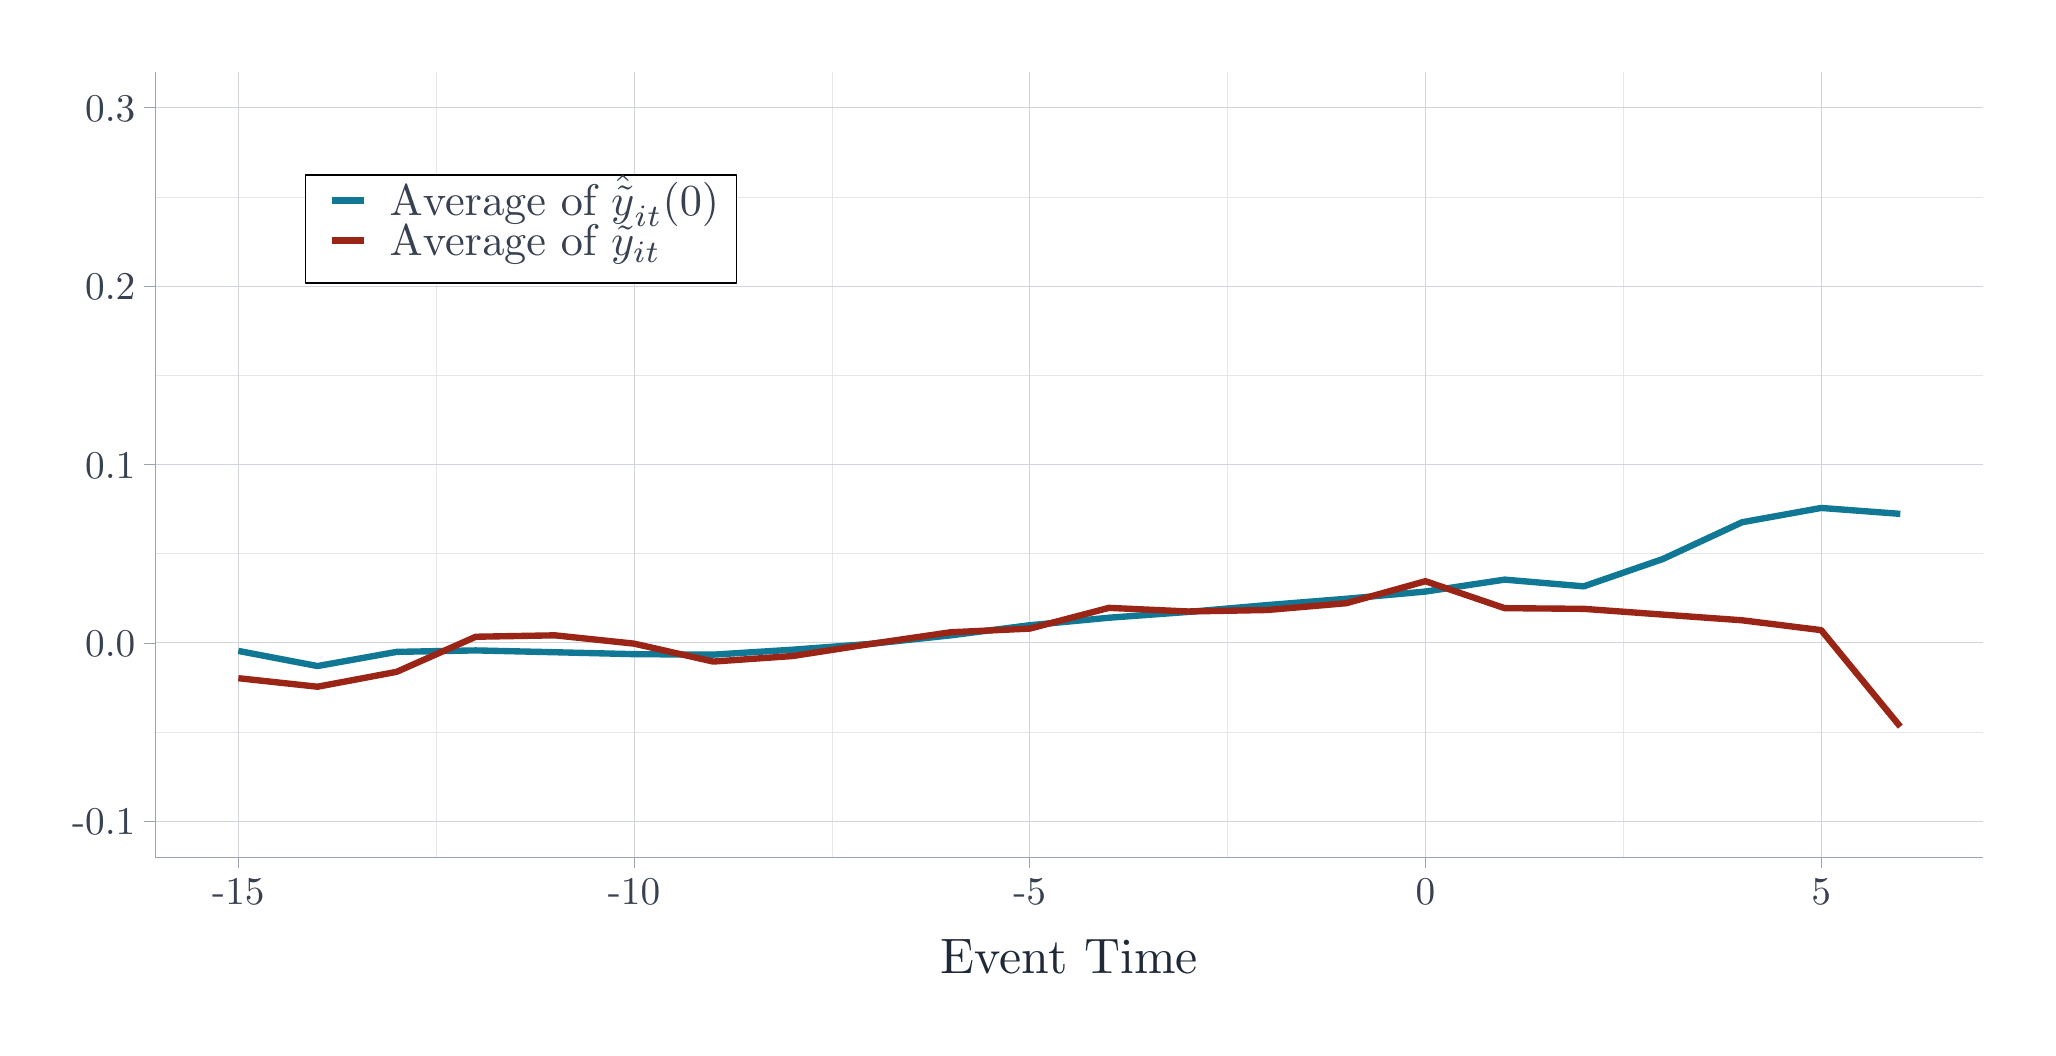
\begin{tikzpicture}[x=1pt,y=1pt]
\definecolor{fillColor}{RGB}{255,255,255}
\path[use as bounding box,fill=fillColor] (0,0) rectangle (722.70,361.35);
\begin{scope}
\path[clip] (  0.00,  0.00) rectangle (722.70,361.35);
\definecolor{drawColor}{RGB}{255,255,255}

\path[draw=drawColor,line width= 0.8pt,line join=round,line cap=round,fill=fillColor] (  0.00,  0.00) rectangle (722.70,361.35);
\end{scope}
\begin{scope}
\path[clip] ( 46.10, 61.65) rectangle (706.70,345.35);
\definecolor{drawColor}{RGB}{255,255,255}
\definecolor{fillColor}{RGB}{255,255,255}

\path[draw=drawColor,line width= 0.8pt,line join=round,line cap=round,fill=fillColor] ( 46.10, 61.65) rectangle (706.70,345.35);
\definecolor{drawColor}{RGB}{229,231,235}

\path[draw=drawColor,line width= 0.2pt,line join=round] ( 46.10,106.79) --
	(706.70,106.79);

\path[draw=drawColor,line width= 0.2pt,line join=round] ( 46.10,171.26) --
	(706.70,171.26);

\path[draw=drawColor,line width= 0.2pt,line join=round] ( 46.10,235.74) --
	(706.70,235.74);

\path[draw=drawColor,line width= 0.2pt,line join=round] ( 46.10,300.22) --
	(706.70,300.22);

\path[draw=drawColor,line width= 0.2pt,line join=round] (147.62, 61.65) --
	(147.62,345.35);

\path[draw=drawColor,line width= 0.2pt,line join=round] (290.61, 61.65) --
	(290.61,345.35);

\path[draw=drawColor,line width= 0.2pt,line join=round] (433.60, 61.65) --
	(433.60,345.35);

\path[draw=drawColor,line width= 0.2pt,line join=round] (576.58, 61.65) --
	(576.58,345.35);
\definecolor{drawColor}{RGB}{209,213,219}

\path[draw=drawColor,line width= 0.4pt,line join=round] ( 46.10, 74.55) --
	(706.70, 74.55);

\path[draw=drawColor,line width= 0.4pt,line join=round] ( 46.10,139.03) --
	(706.70,139.03);

\path[draw=drawColor,line width= 0.4pt,line join=round] ( 46.10,203.50) --
	(706.70,203.50);

\path[draw=drawColor,line width= 0.4pt,line join=round] ( 46.10,267.98) --
	(706.70,267.98);

\path[draw=drawColor,line width= 0.4pt,line join=round] ( 46.10,332.45) --
	(706.70,332.45);

\path[draw=drawColor,line width= 0.4pt,line join=round] ( 76.13, 61.65) --
	( 76.13,345.35);

\path[draw=drawColor,line width= 0.4pt,line join=round] (219.12, 61.65) --
	(219.12,345.35);

\path[draw=drawColor,line width= 0.4pt,line join=round] (362.10, 61.65) --
	(362.10,345.35);

\path[draw=drawColor,line width= 0.4pt,line join=round] (505.09, 61.65) --
	(505.09,345.35);

\path[draw=drawColor,line width= 0.4pt,line join=round] (648.08, 61.65) --
	(648.08,345.35);
\definecolor{drawColor}{RGB}{16,120,149}

\path[draw=drawColor,line width= 2.3pt,line join=round] ( 76.13,136.14) --
	(104.73,130.67) --
	(133.33,135.79) --
	(161.92,136.32) --
	(190.52,135.66) --
	(219.12,134.97) --
	(247.71,134.79) --
	(276.31,136.57) --
	(304.91,138.71) --
	(333.51,141.76) --
	(362.10,145.42) --
	(390.70,148.13) --
	(419.30,150.22) --
	(447.90,152.70) --
	(476.49,154.98) --
	(505.09,157.59) --
	(533.69,161.90) --
	(562.28,159.47) --
	(590.88,169.35) --
	(619.48,182.63) --
	(648.08,187.80) --
	(676.67,185.66);
\definecolor{drawColor}{RGB}{154,36,21}

\path[draw=drawColor,line width= 2.3pt,line join=round] ( 76.13,126.28) --
	(104.73,123.20) --
	(133.33,128.58) --
	(161.92,141.26) --
	(190.52,141.77) --
	(219.12,138.77) --
	(247.71,132.29) --
	(276.31,134.28) --
	(304.91,138.71) --
	(333.51,142.88) --
	(362.10,144.20) --
	(390.70,151.70) --
	(419.30,150.39) --
	(447.90,150.92) --
	(476.49,153.38) --
	(505.09,161.33) --
	(533.69,151.59) --
	(562.28,151.34) --
	(590.88,149.26) --
	(619.48,147.21) --
	(648.08,143.65) --
	(676.67,108.77);

\path[] ( 46.10, 61.65) rectangle (706.70,345.35);
\end{scope}
\begin{scope}
\path[clip] (  0.00,  0.00) rectangle (722.70,361.35);
\definecolor{drawColor}{RGB}{156,163,175}

\path[draw=drawColor,line width= 0.3pt,line join=round] ( 46.10, 61.65) --
	( 46.10,345.35);
\end{scope}
\begin{scope}
\path[clip] (  0.00,  0.00) rectangle (722.70,361.35);
\definecolor{drawColor}{RGB}{55,65,81}

\node[text=drawColor,anchor=base east,inner sep=0pt, outer sep=0pt, scale=  1.42] at ( 38.90, 69.65) {-0.1};

\node[text=drawColor,anchor=base east,inner sep=0pt, outer sep=0pt, scale=  1.42] at ( 38.90,134.13) {0.0};

\node[text=drawColor,anchor=base east,inner sep=0pt, outer sep=0pt, scale=  1.42] at ( 38.90,198.61) {0.1};

\node[text=drawColor,anchor=base east,inner sep=0pt, outer sep=0pt, scale=  1.42] at ( 38.90,263.08) {0.2};

\node[text=drawColor,anchor=base east,inner sep=0pt, outer sep=0pt, scale=  1.42] at ( 38.90,327.56) {0.3};
\end{scope}
\begin{scope}
\path[clip] (  0.00,  0.00) rectangle (722.70,361.35);
\definecolor{drawColor}{RGB}{156,163,175}

\path[draw=drawColor,line width= 0.3pt,line join=round] ( 42.10, 74.55) --
	( 46.10, 74.55);

\path[draw=drawColor,line width= 0.3pt,line join=round] ( 42.10,139.03) --
	( 46.10,139.03);

\path[draw=drawColor,line width= 0.3pt,line join=round] ( 42.10,203.50) --
	( 46.10,203.50);

\path[draw=drawColor,line width= 0.3pt,line join=round] ( 42.10,267.98) --
	( 46.10,267.98);

\path[draw=drawColor,line width= 0.3pt,line join=round] ( 42.10,332.45) --
	( 46.10,332.45);
\end{scope}
\begin{scope}
\path[clip] (  0.00,  0.00) rectangle (722.70,361.35);
\definecolor{drawColor}{RGB}{156,163,175}

\path[draw=drawColor,line width= 0.3pt,line join=round] ( 46.10, 61.65) --
	(706.70, 61.65);
\end{scope}
\begin{scope}
\path[clip] (  0.00,  0.00) rectangle (722.70,361.35);
\definecolor{drawColor}{RGB}{156,163,175}

\path[draw=drawColor,line width= 0.3pt,line join=round] ( 76.13, 57.65) --
	( 76.13, 61.65);

\path[draw=drawColor,line width= 0.3pt,line join=round] (219.12, 57.65) --
	(219.12, 61.65);

\path[draw=drawColor,line width= 0.3pt,line join=round] (362.10, 57.65) --
	(362.10, 61.65);

\path[draw=drawColor,line width= 0.3pt,line join=round] (505.09, 57.65) --
	(505.09, 61.65);

\path[draw=drawColor,line width= 0.3pt,line join=round] (648.08, 57.65) --
	(648.08, 61.65);
\end{scope}
\begin{scope}
\path[clip] (  0.00,  0.00) rectangle (722.70,361.35);
\definecolor{drawColor}{RGB}{55,65,81}

\node[text=drawColor,anchor=base,inner sep=0pt, outer sep=0pt, scale=  1.42] at ( 76.13, 44.66) {-15};

\node[text=drawColor,anchor=base,inner sep=0pt, outer sep=0pt, scale=  1.42] at (219.12, 44.66) {-10};

\node[text=drawColor,anchor=base,inner sep=0pt, outer sep=0pt, scale=  1.42] at (362.10, 44.66) {-5};

\node[text=drawColor,anchor=base,inner sep=0pt, outer sep=0pt, scale=  1.42] at (505.09, 44.66) {0};

\node[text=drawColor,anchor=base,inner sep=0pt, outer sep=0pt, scale=  1.42] at (648.08, 44.66) {5};
\end{scope}
\begin{scope}
\path[clip] (  0.00,  0.00) rectangle (722.70,361.35);
\definecolor{drawColor}{RGB}{31,41,55}

\node[text=drawColor,anchor=base,inner sep=0pt, outer sep=0pt, scale=  1.80] at (376.40, 19.50) {Event Time};
\end{scope}
\begin{scope}
\path[clip] (  0.00,  0.00) rectangle (722.70,361.35);
\definecolor{drawColor}{RGB}{0,0,0}
\definecolor{fillColor}{RGB}{255,255,255}

\path[draw=drawColor,line width= 0.6pt,line join=round,line cap=round,fill=fillColor] (100.36,269.16) rectangle (256.09,308.06);
\end{scope}
\begin{scope}
\path[clip] (  0.00,  0.00) rectangle (722.70,361.35);
\definecolor{drawColor}{RGB}{255,255,255}
\definecolor{fillColor}{RGB}{255,255,255}

\path[draw=drawColor,line width= 0.8pt,line join=round,line cap=round,fill=fillColor] (108.36,291.61) rectangle (122.81,306.06);
\end{scope}
\begin{scope}
\path[clip] (  0.00,  0.00) rectangle (722.70,361.35);
\definecolor{drawColor}{RGB}{16,120,149}

\path[draw=drawColor,line width= 2.3pt,line join=round] (109.81,298.84) -- (121.37,298.84);
\end{scope}
\begin{scope}
\path[clip] (  0.00,  0.00) rectangle (722.70,361.35);
\definecolor{drawColor}{RGB}{255,255,255}
\definecolor{fillColor}{RGB}{255,255,255}

\path[draw=drawColor,line width= 0.8pt,line join=round,line cap=round,fill=fillColor] (108.36,277.16) rectangle (122.81,291.61);
\end{scope}
\begin{scope}
\path[clip] (  0.00,  0.00) rectangle (722.70,361.35);
\definecolor{drawColor}{RGB}{154,36,21}

\path[draw=drawColor,line width= 2.3pt,line join=round] (109.81,284.38) -- (121.37,284.38);
\end{scope}
\begin{scope}
\path[clip] (  0.00,  0.00) rectangle (722.70,361.35);
\definecolor{drawColor}{RGB}{55,65,81}

\node[text=drawColor,anchor=base west,inner sep=0pt, outer sep=0pt, scale=  1.60] at (130.81,293.33) {Average of $\hat{\tilde{y}}_{it}(0)$};
\end{scope}
\begin{scope}
\path[clip] (  0.00,  0.00) rectangle (722.70,361.35);
\definecolor{drawColor}{RGB}{55,65,81}

\node[text=drawColor,anchor=base west,inner sep=0pt, outer sep=0pt, scale=  1.60] at (130.81,278.87) {Average of $\tilde{y}_{it}$};
\end{scope}
\end{tikzpicture}
